\citep{davidson2022hypersphericalvariationalautoencoders} propose an algorithm to sample
a $\text{vMF}(\mathbf{\boldsymbol{\mu}}, \kappa)$ random variable that relies on rejection sampling.
This has obvious speed limitations and as such I sought out to understand how much faster
it is to sample a SphericalTNBBeta random variable on a single GPU. \Cref{fig:speed-heatmap}
shows that SphericalTNBBeta sampling is at least twice as fast as vMF sampling, and
depending on the latent dimension, batch size, and concentration parameter, this ratio
dramatically increases.
\begin{figure}[H]
    \centering
    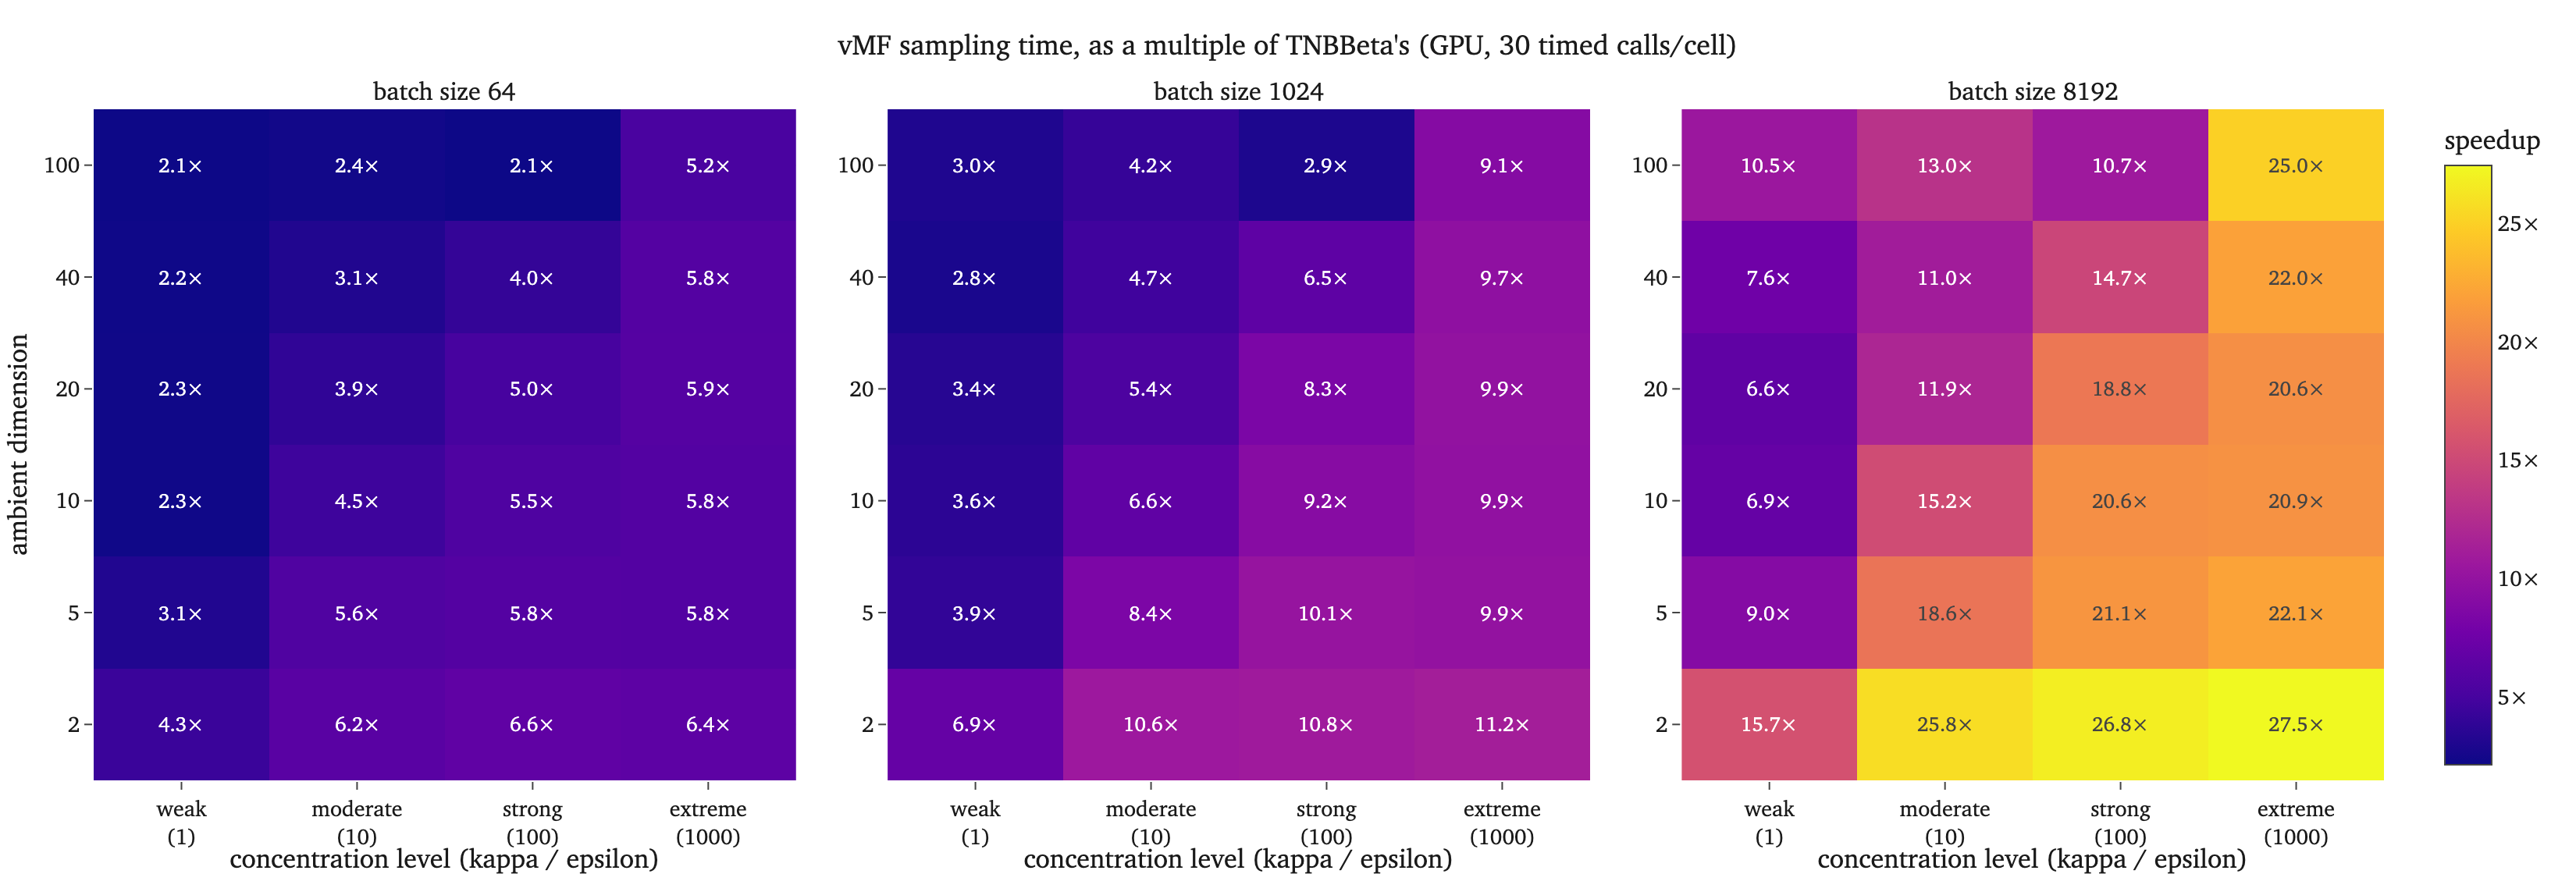
\includegraphics[width=\linewidth]{assets/sampling_speed_heatmap.png}
    \caption{Comparison of sampling runtime between SphericalTNBBeta and vMF distributions.}
    \label{fig:speed-heatmap}
\end{figure}
To understand where the TNBBeta sits in relation to the vMF and Gaussian VAEs, I replicated
table 1 from \citep{davidson2022hypersphericalvariationalautoencoders}, this time adding the
TNBBeta-VAE's results. Namely, I trained a series of VAEs on binarized MNIST using a
convolutional\footnote{Implementation details can be found here: https://github.com/Dant86/tnbbeta\_vae}
encoder and decoder. \Cref{tab:mnist-table1} outlines performance on the test set over varying
latent dimensions. Note that $d$ denotes the manifold dimension in line with the reference
paper's methodology. In particular, a spherical embedding for $d=2$ lies in $\mathbb{S}^2 \subset \mathbb{R}^3$.

\begin{table}[H]
    \centering
    \resizebox{\textwidth}{!}{%
    \begin{tabular}{lcccccccccccc}
        \toprule
        & \multicolumn{4}{c}{N-VAE} & \multicolumn{4}{c}{vMF} & \multicolumn{4}{c}{SphericalTNBBeta} \\
        \cmidrule(lr){2-5} \cmidrule(lr){6-9} \cmidrule(lr){10-13}
        $d$ & LL & $\mathcal{L}[q]$ & RE & KL & LL & $\mathcal{L}[q]$ & RE & KL & LL & $\mathcal{L}[q]$ & RE & KL \\
        \midrule
        2  & $-132.64_{\pm 0.30}$ & $-136.81_{\pm 0.28}$ & $-129.19_{\pm 0.35}$ & $7.62_{\pm 0.10}$ & $-130.86_{\pm 0.43}$ & $-134.42_{\pm 0.42}$ & $-126.89_{\pm 0.47}$ & $7.53_{\pm 0.08}$ & $-130.11_{\pm 0.57}$ & $-134.21_{\pm 0.46}$ & $-126.43_{\pm 0.54}$ & $7.78_{\pm 0.11}$ \\
        5  & $-105.38_{\pm 0.11}$ & $-109.53_{\pm 0.09}$ & $-96.12_{\pm 0.12}$ & $13.41_{\pm 0.17}$ & $-105.27_{\pm 0.14}$ & $-109.32_{\pm 0.08}$ & $-95.56_{\pm 0.12}$ & $13.76_{\pm 0.06}$ & $-104.89_{\pm 0.22}$ & $-109.15_{\pm 0.22}$ & $-95.36_{\pm 0.26}$ & $13.79_{\pm 0.13}$ \\
        10 & $\mathbf{-88.75_{\pm 0.12}}$ & $\mathbf{-92.91_{\pm 0.14}}$ & $-72.38_{\pm 0.10}$ & $20.53_{\pm 0.12}$ & $-89.38_{\pm 0.02}$ & $-93.60_{\pm 0.06}$ & $-71.84_{\pm 0.08}$ & $21.77_{\pm 0.05}$ & $-89.29_{\pm 0.10}$ & $-93.65_{\pm 0.14}$ & $-71.96_{\pm 0.25}$ & $21.69_{\pm 0.14}$ \\
        20 & $\mathbf{-83.67_{\pm 0.09}}$ & $\mathbf{-87.64_{\pm 0.11}}$ & $-61.87_{\pm 0.14}$ & $25.77_{\pm 0.07}$ & $-86.84_{\pm 0.04}$ & $-92.10_{\pm 0.05}$ & $-62.63_{\pm 0.21}$ & $29.47_{\pm 0.18}$ & $-86.90_{\pm 0.23}$ & $-92.12_{\pm 0.15}$ & $-62.33_{\pm 0.41}$ & $29.78_{\pm 0.53}$ \\
        40 & $-83.24_{\pm 0.05}$ & $-87.40_{\pm 0.07}$ & $-60.77_{\pm 0.11}$ & $26.63_{\pm 0.14}$ & $-144.28_{\pm 31.06}$ & $-170.06_{\pm 41.29}$ & $-162.32_{\pm 56.08}$ & $7.73_{\pm 14.79}$ & $-89.09_{\pm 0.15}$ & $-96.38_{\pm 0.14}$ & $-62.53_{\pm 0.42}$ & $33.86_{\pm 0.36}$ \\
        \bottomrule
    \end{tabular}%
    }
    \caption{Reproduction on binarized MNIST (conv encoder/decoder, 500-sample
        importance-weighted test log-likelihood, 5 seeds). N-VAE is the Gaussian baseline.
        $\mathcal{L}[q]$ is the ELBO, RE the reconstruction term, KL the exact KL
        (Gaussian, vMF) or a Monte Carlo estimate (TNBBeta, no closed form). \textbf{Bold}
        = best mean in the row, significant at $p < 0.01$ (Welch's $t$-test).}
    \label{tab:mnist-table1}
\end{table}
We see that for low dimensions, the vMF and SphericalTNBBeta VAEs perform similarly both in terms
of reconstruction error and KL. The vMF VAE becomes unstable in higher dimensions ($d=40$) and as such its
performance degrades, and while Gaussian is the clear winner, there's no sharp drop in performance for the
TNBBeta-VAE.

The fact that the S-VAE and TNBBeta-VAE perform similarly in low dimensions begs the question:
are the respective latent posteriors similar? A quick glance at the latent embeddings in the style
of \citep{davidson2022hypersphericalvariationalautoencoders} could give some signal:
\begin{figure}[H]
    \centering
    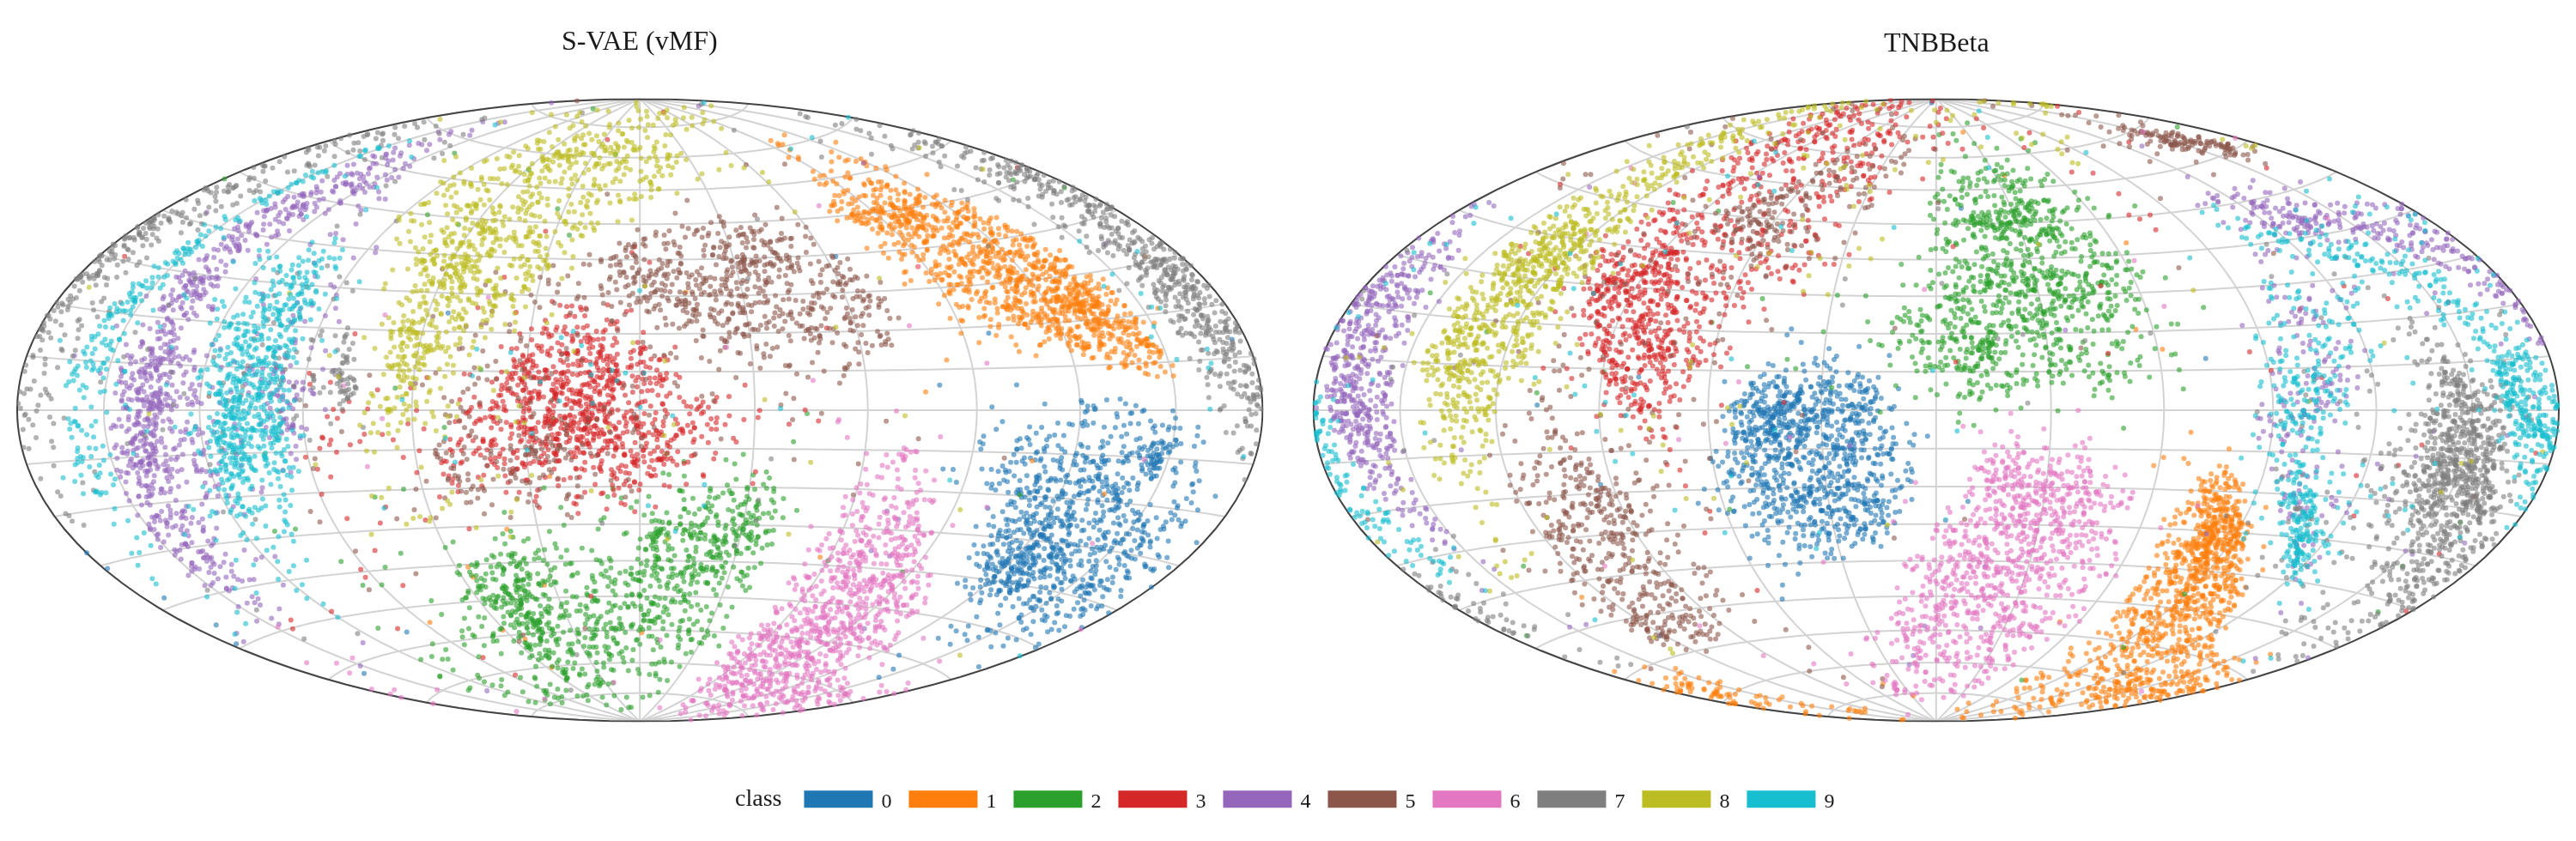
\includegraphics[width=\textwidth]{assets/hammer_mnist_vmfs_d2_seed0_vs_mnist_tnbs_d2_seed0.png}
    \caption{Hammer projection of latent embeddings in the S-VAE and TNBBeta-VAE trained on MNIST with $d=2$.}
    \label{fig:hammer}
\end{figure}
One very striking observation from the above is that both VAEs arrange MNIST class embeddings within
cap-like clusters on the unit hypersphere. Based on the distribution heatmaps from \Cref{fig:ablations}
I found the observation for the TNBBeta-VAE quite striking: the heatmaps show that, depending on the
parameters $p, q, \varepsilon$, mass is often concentrated about a ring on the unit hypersphere
as opposed to a cap. While running these experiments I often noticed that the SphericalTNBBeta posterior
would often converge to $p \to 1, q \to 0$ (see the bottom-left corner
of \Cref{fig:pq-ablation}) which does in fact concentrate mass about a cap, and not a ring. To verify this in higher dimensions,
I attempted to quantify ``ring-ness''. Claude Sonnet 5 suggested running an experiment to determine whether any mass
per MNIST class was distributed about a ring at all. 

\Cref{tab:ring-exclusion} includes the first diagnostic I used to determine whether any MNIST classes'
embeddings were distributed about a cap on the unit hypersphere. The "far-side \%" metric is computed
as follows: for each MNIST class, we compute the centroid embedding, and calculate the percent of
embeddings across the test set within that class that have negative cosine similarity to the
centroid. The ``antipodal \%" metric is calculated similarly, but we instead calculate the percent of
embeddings that have cosine similarity less than -0.9. This percentage is then averaged across all classes
for both metrics.
\begin{table}[H]
\centering
\begin{tabular}{lcccc}
\toprule
& \multicolumn{2}{c}{Far-side (\%)} & \multicolumn{2}{c}{Antipodal (\%)} \\
\cmidrule(lr){2-3} \cmidrule(lr){4-5}
$d$ & S-VAE (vMF) & TNBBeta & S-VAE (vMF) & TNBBeta \\
\midrule
2  & 1.56 $\pm$ 0.29 & 2.16 $\pm$ 0.71 & 0.12 $\pm$ 0.02 & 0.12 $\pm$ 0.05 \\
5  & 0.39 $\pm$ 0.04 & 0.37 $\pm$ 0.04 & 0.00 $\pm$ 0.00 & 0.00 $\pm$ 0.00 \\
10 & 0.52 $\pm$ 0.05 & 0.52 $\pm$ 0.04 & 0.00 $\pm$ 0.00 & 0.00 $\pm$ 0.00 \\
20 & 1.77 $\pm$ 0.11 & 1.77 $\pm$ 0.10 & 0.00 $\pm$ 0.00 & 0.00 $\pm$ 0.00 \\
40 & 3.00 $\pm$ 0.14 & 2.83 $\pm$ 0.06 & 0.00 $\pm$ 0.00 & 0.00 $\pm$ 0.00 \\
\bottomrule
\end{tabular}
\caption{Ring-shape check: percentage of each class's points more than
$90^\circ$ (respectively, within $0.9$ cosine of the exact antipode) from their own
class's centroid direction. Mean $\pm$ std over 5 seeds.}
\label{tab:ring-exclusion}
\end{table}
If the mass of each class-conditional distribution is, in fact, concentrated about a cap, then
one expects both metrics above to be extremely low: all embeddings should align closely with
the centroid. If ``far-side \%'' is high and ``antipodal \%'' is low, then we have reason to
believe that the class embeddings form a ring-like distribution. Based on the above results, though,
there is no evidence to believe that such a ring-like structure is ever taken on.